\chapter{Design}
\label{chap:Design}
% 9 pages
After reviewing related previous studies, this chapter will discuss various possible designs and rationales for the system design before actual implementation according to project requirements.

Firstly, the design of the data collection process is introduced in section \ref{sec:Data set collection}, including the data type to be collected, the labelling approach and the functionalities that need to be implemented in the data collection app.

Secondly, it is necessary to design the data preprocessing pipeline in section \ref{sec:Data preprocessing} according to the anonymity requirement detailed in research ethics (section \ref{sec:Research ethics}), and transform the data to make it suitable for model input.

Thirdly, the design of a deep model suitable for solving the problem of this research is detailed in section \ref{sec:Deep model design}, based on the related previous research and the background of deep models.

\section{Data set collection}
\label{sec:Data set collection}
In section \ref{sec:Data features and classic methods}, I have reviewed feature engineering and classic machine learning models before deep learning was widely used.
They are extremely helpful for designing data sets collection guidelines for human action recognition tasks and designing a deep model.

\subsection{Requirements of data set}
The main difficulty of human action recognition tasks is exactly the same difficulty in the superset of them -- video understanding.

It is difficult to obtain enough data in both number and quality to train deep-learning models, especially for a video data set.

There are many public data sets for video understanding, but unfortunately, none of them has the video types needed within the research objectives.

\subsection{Functionality of data collection web-app}
 % 2.5 pages

\section{Data preprocessing}
\label{sec:Data preprocessing} % 1 page
After collecting videos uploaded by participants to create a video data set, data preprocessing is the next process of adjusting the data to meet the research ethics requirements processing it into an input format suitable for the model data loader.
The encoding format of video recorded in the browser is WebP, a highly compressed video format developed by Google.
If the model data loader decodes the video data during the training process, it will consume lots of CPU during the decompression and anonymisation process.

An optimisation method is decoding the video into a sequence of pictures in the data preprocessing process to reduce the computational overhead in the training process.
An anonymous algorithm will be applied to each frame and save the results in picture format.
In this way, the data loader only needs to load the processed pictures during the training process.

According to research ethics requirements, the data preprocessing process will use an anonymisation algorithm to minimise the presence of facial details that might enable the identification of an individual.
The anonymisation algorithm cannot directly mask the face completely.
Because the facial information contains many features that help the model to classify activities, such as the direction of sight, the lip movement during speaking, etc.

The anonymisation algorithm should strike a balance between the complexity of implementation, performance, and the ability to keep research related facial features.
In the research, a simple two-step algorithm, namely feature masked face concealment, is used to extract the key facial features while covering the other facial areas.

The following two subsections will introduce the details of the two-step process in the anonymisation algorithm.
The first step is to find and locate faces in the video, and the second step is to extract facial feature points and perform masking on each frame.

\subsection{Face detection with Viola--Jones algorithm} % 1 page
\citet{viola2001rapid} proposed a fast object detection approach using Haar-like features, namely Viola--Jones algorithm, which extracts features from input images using a series of adjacent rectangular regions.
This operation is very similar to the convolution operation in convolutional neural networks.
However, the difference is that the proposed Haar Cascade uses predefined feature extraction kernels, such as edge features, line features, etc.
The classifier part uses AdaBoost algorithm, a famous Boosting method in ensemble learning, in which it trains many weak classifiers to form a more accurate strong classifier.

Currently, this algorithm is very mature and has been widely used in many studies.
For example, a previous study of virtual exam controller proposed by \citet{garg2020convolutional} was introduced early in the literature review section \ref{sec:Online exam security system}.
In this case, they use Haar Cascade Classifier to detect, tag, and identify the students face and using deep learning to apply exam constraints.

Technically, Haar Cascade Classifier use cascade structure to form multiple stages to classify face regions as shown in Figure \ref{fig:ext-haar-arch}.
This classifier has four vital features that enable it to be widely used in face detection tasks quickly, summarised by \citet{garg2020convolutional} as follows:

\begin{minipage}{\textwidth}
    \begin{minipage}{.4\textwidth}
        \begin{itemize}
            \item Using Haar-like features.
            \item Using the integral picture.
            \item Using AdaBoost learning.
            \item Using cascading classifiers.
        \end{itemize}
    \end{minipage}
    \begin{minipage}{.58\textwidth}
        \centering
        \captionsetup{type=figure}
        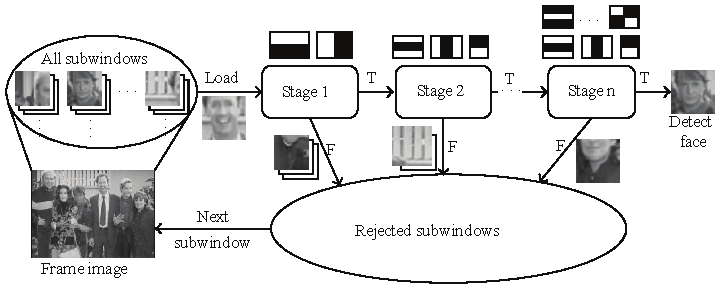
\includegraphics[width=\textwidth]{design/imgs/ext-haar-arch.pdf}
        \captionof{figure}{Haar Cascade structure \cite{kim2015system}}
        \label{fig:ext-haar-arch}
    \end{minipage}
\end{minipage}

OpenCV has provided a good implementation, cv::CascadeClassifier\footnote{cascadedetect.cpp: \url{https://github.com/opencv/opencv/tree/4.5.3/modules/objdetect/src}} and a variety of trained models\footnote{Available models: \url{https://github.com/opencv/opencv/tree/4.5.3/data/haarcascades}} for selection.
In addition, the API design for this module is clear and easy to use.
The trained model can be loaded through cv::CascadeClassifier::load method, and then cv::CascadeClassifier::detectMultiScale can be used to locate the face positions in the input image and return the result of faces in the format of rectangular areas.

To summary, this Haar Cascade object detection method is suitable for real-time face detection on mobile devices with the advantage of requiring a small amount of calculation. 
Therefore, this research will use this method to perform the face detection procedure in the anonymisation algorithm.

\subsection{Face landmark extraction and face concealment} % 1 page
As mentioned above, after obtaining the position of faces from the input video, it also needs to extract face landmark points and overlay them on the top after masking face details.

A highly efficient and accurate face alignment algorithm was proposed by \citet{ren2014face} in 2014.
This research still uses classic machine learning methods for low computation complexity by using a combination of random forest and global linear regression to regress key points of facial features.
It learns the local binary features (LBF) of each key point through random forest, then combines the features and uses linear regression to obtain the key points.
A facial landmark detection survey study published by \citet{wu2019facial} concluded that this regression-based method has both good performance and fast speed.

\begin{figure}[!ht]
    \centering
    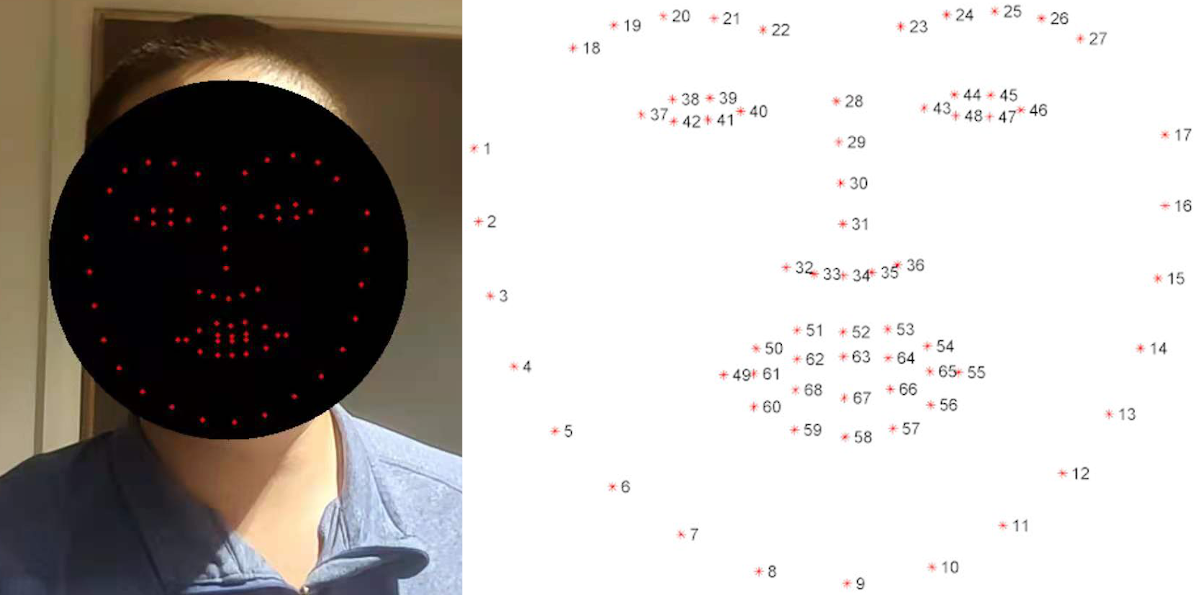
\includegraphics[width=\textwidth]{design/imgs/3-face-landmark.png}
    \caption{Landmark masked face concealment and face landmark schematic}
    \label{fig:3-face-landmark}
\end{figure}

The left picture in Figure \ref{fig:3-face-landmark} illustrates an exemplar face image (anonymised result) with landmark masked face concealment applied.
The right side in the figure displays the schematic of the face landmarks used in this research.
The schematic has 68 key points to locate face landmarks in the image.
These key points can represent many facial features, such as face orientation, lips movement and other details without exposing unrelated details in classifying exam activity.

In OpenCV, this algorithm is also implemented in extra contrib modules.
The class of detecting face landmarks with LBF algorithm is defined in cv::face::FacemarkLBF\footnote{facemarkLBF.cpp: \url{https://github.com/opencv/opencv_contrib/blob/4.5.3/modules/face/src}}, and the corresponding trained model\footnote{LBF model: \url{https://github.com/kurnianggoro/GSOC2017/raw/master/data/lbfmodel.yaml}} is provided by the algorithm contributors.
In addition, the algorithm implementation inherits the simple and easy-to-use API of the object detection framework in OpenCV.
Generally, using FacemarkLBF::loadModel method to load trained model and FacemarkLBF::setFaceDetector to set a custom face detector function where Haar Cascade will firstly detect face regions in the input image.
 % 3 pages

\section{Deep model design}
\label{sec:Deep model design}
Since deep networks have the duties of feature extraction, deep learning methods no longer require manual feature engineering.
But it is still necessary to consider that different deep networks have inductive biases (preferences) for different feature types.
The literature review section \ref{sec:Deep models detail} has reviewed models detail and instinct properties.
For example, CNN has properties of translation invariance and is suitable for imagery features; Transformers has properties of long-range dependency modelling and adapts to time-series features.

The model design procedure includes not only the network architecture but also the data loader.
The latter is responsible for reading the result from the previous data pre-processing procedure and transforming them into the tensor shapes required by the model input layer.
Because the data loader is the foremost part of the model design, this section will begin with the detail of loading data.
Then, the deep network architecture for the research goal will be detailed, as well as the output layer for generating probability results.

\subsection{Data loader and input layer}
The data loader is a binding bridge between the processed data set and the model input layer, which converts the data format from the former into information that the model's input layer can accept.
As discussed in pre-processing section \ref{sec:Data preprocessing}, the results from the previous procedure are individual video frames saved in picture format.
Thus, any picture library in Python can read the inputs into memory, such as OpenCV, which was also previously used in data pre-processing.

Table \ref{tab:Model input tensors} shows the design of tensors of the model's input layer.
The model needs to input these two tensors in each step in training or inference.
The first tensor in the table represents the image sequence, and the second tensor describes the frame position in the image sequence corresponding to the original video clip.

\begin{table}[!ht]
\renewcommand{\arraystretch}{1.2}
\begin{tabularx}{\textwidth}{|c|c|c|X|}
\hline
Tensor ID & Name           & Shape                    & Description                                            \\ \hline
0         & Images   & {[}1, 3, 16, 224, 224{]} & {[}Batch size, RGB channels, Frames, Height, Weight{]} \\ \hline
1         & Positions & {[}1, 16{]}              & {[}Batch size, Frame position{]}                       \\ \hline
\end{tabularx}
\caption{Model input tensors}
\label{tab:Model input tensors}
\end{table}

In detail, the first tensor represents the image sequence, which is a five-dimensional array defined in tensor shape.
The first number of this tensor shape is batch size, which represents the number of samples utilised in one iteration.
Usually, in the model training process, the batch size should be increased as much as possible under the resource allowance of the hardware so that more samples can be taken into account when calculating the back-prorogation gradient and avoid over-fitting.
In the inference process after model training and deployment, the batch size is always one.
The second part of the tensor shape is channels, which represents the three channels of red, green and blue in the case of an RGB image.
The third number in the tensor shape is the number of frames uniformly sampled from the video.
The last two numbers in tensor shape are the height and width of the image.

The second tensor represents the frame position number in the video clip.
This position number will be used as position embedding in the temporal backbone network to capture the temporal features.
A larger number of frames in one iteration can give more data to the model, improve the accuracy and the ability to predict long-term activities, but it also requires longer capture time and computing resources.
To strike a balance between the model performance and resources required, I define the number of frames and frame positions in each iteration to be 16 in this study.

\subsection{The model architecture}
After the data loader converts the input data into a suitable format for the input layer, the next step is to select a spatial backbone and a temporal backbone, then design a data flow to connect them in the model architecture.
The block flowchart in Figure \ref{fig:3-model-dataflow} shows the data flow from the input layer through spatial and temporal deep networks to the final category possibility output.

\begin{wrapfigure}[19]{r}{.32\textwidth}
    \vspace*{-1.2em}
    \centering
    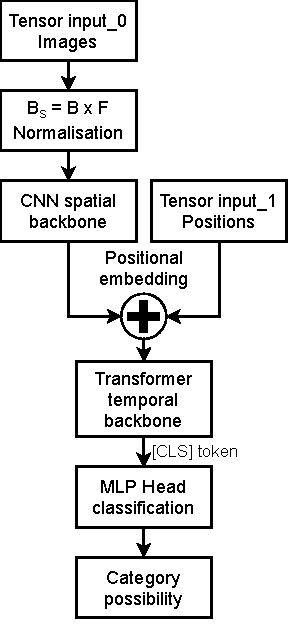
\includegraphics[width=.32\textwidth]{design/imgs/3-model-dataflow.pdf}
    \caption{The data flow}
    \label{fig:3-model-dataflow}
\end{wrapfigure}

As for the spatial backbone, this research uses a minimal EfficientNet-B0 backbone pre-trained on the ImageNet data set to do spatial feature extraction from frames.
The detail and evolution history of EfficientNet is reviewed in subsection  \ref{subsec:Evolution from MobileNet to EfficientNet}.
To summary, it is a further optimisation from MobileNet, also a CNN deep network designed for mobile devices.

As for the temporal backbone, Longformer is used in this research as a temporal encoder with global attention in \textit{[CLS] token} and local sliding window attention pattern.
In subsection \ref{subsec:Optimisation of Transformer Networks}, many previous studies have pointed out the high computational complexity of the self-attention mechanism in Transformer, and proposed corresponding improvements to facilitate running on mobile devices.

The output layer receives hidden states of the \textit{[CLS] token} from the Transformer-based temporal encoder and outputs the normalised category probability.
This research uses two fully connected dense layers as the multiple layer perceptron classification header reviewed in Figure \ref{fig:ext-vtn}, Video Transformer Network architecture.

The output dimension of the first dense layer is equal to the output shape of the temporal encoder, and a Gaussian Error Linear Unit (GELU) is used for nonlinear activation mapping.
The final output layer dimension of the model is the number of classification categories.

In this study, considering the difficulty of data set collection, 12 activities were designed in \ref{sec:Output categories} Table \ref{tab:Model output}, covering the common types of remote exams.
This table also contains related descriptions and predefined risk levels for each activity, expressed in three alert levels.

\subsection{Loss function and training hyperparameters}
\label{subsec:Loss function and training hyperparameters}
The categorical crossentropy loss is a commonly used loss function in classification tasks.
In TensorFlow, if the labels is in one-hot representation, \textit{CategoricalCrossentropy} loss should be used.
In the case of labels provided as integers, \textit{SparseCategoricalCrossentropy} should be used.
Since this study uses a deep learning model to solve the multi-classification problem where the label of each data sample is a integer category index of the matching category, the appropriate loss function is \textit{tf.keras.losses.SparseCategoricalCrossentropy}.

Many hyperparameters are involved in the deep model training process, where the model performance is closely related to fine-tuning.
The process of training any deep model involves two important hyperparameters, batch size and learning rate.
The batch size represents the number of samples input to the model in each iteration.
The learning rate represents the update factor of the model weight moving toward a minimum of the loss function.
A larger batch size allows the trainer to better calculate the back-propagation gradient with more samples, where appropriately increasing the learning rate can make the model converge faster.
A too-large learning rate will cause an oscillating loss value making the model difficult to converge.
Conversely, a too-small learning rate will slow down the training process and make the optimiser easier to get stuck at saddle points.

Because the Transformer has high versatility and low inductive bias than CNN, many previous studies have shown that learning rate warm-up is an effective and necessary design to prevent over-fitting when training Transformer-based deep networks.
An intuitive explanation for the learning rate warm-up is that the model knows nothing about the data attributes and distribution at the beginning of training.
Using a large learning rate at the beginning will cause the model to over-fit the first few samples immediately, making it hard to remedy it in the subsequent training steps.

Equation \ref{eq:lr-schedule} shows the learning rate scheduler function, where $d_{model}$ defines the maximum learning rate applicable to the model complexity, and $step\_num$ defines the number of iterations to reach the peak learning rate.

\begin{equation}
    lrate=d_{model}^{-0.5} * \min \left(step\_num^{-0.5}, step\_num \cdot  warmup\_steps^{-1.5}\right)
    \eqcite{vaswani2017attention}
    \label{eq:lr-schedule}
\end{equation}

There are many more hyperparameters other than the learning rate for the training process, but they are less important than hyperparameters that directly controlling the model complexity and the training process.
For example, some hyperparameters used in data augmentation -- scaling factors, cropping ranges and possibilities for each augmentation operation.
Stronger data augmentation can better prevent overfitting but may introduce more noises in the training process.
To reduce the search space for hyperparameter fine-tuning, this study reviews the implementation of related researches to set those less impactful hyperparameters.
 % 3 pages